\begin{figure}[H]
    \centering
    \label{fig:comp-graph-example}
    
    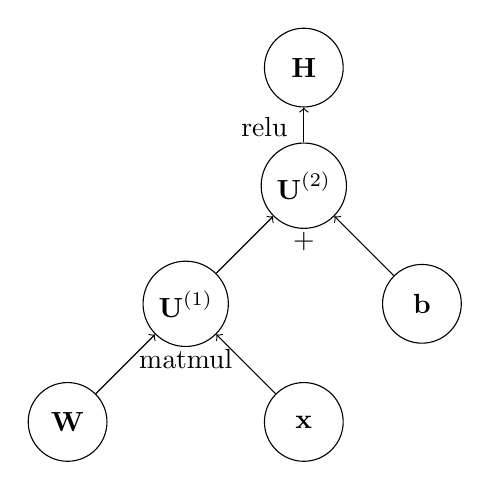
\begin{tikzpicture}
        \def\vert{1.5}
        \def\hori{1.5}
        \tikzstyle{place}=[circle, draw=black, minimum size=10mm]
        
        % Nodes
        \node[place] (w) at (0 * \hori, 0 * \vert) {\textbf{W}};
        \node[place] (x) at (2 * \hori, 0 * \vert) {\textbf{x}};
        
        \node[place, label={[shift={(0.0,-1.5)}]{\text{matmul}}}] (u1) at (1 * \hori, 1 * \vert) {$\textbf{U}^{(1)}$};
        \node[place] (b) at (3 * \hori, 1 * \vert) {\textbf{b}};
        
        
        \node[place, label={[shift={(0.0,-1.5)}]{\text{+}}}] (u2) at (2 * \hori, 2 * \vert) {$\textbf{U}^{(2)}$};
        
        \node[place, label={[shift={(-0.5,-1.5)}]{\text{relu}}}] (h) at (2 * \hori, 3 * \vert) {\textbf{H}};
        
        % Edges
        \draw [->] (w) to (u1);
        \draw [->] (x) to (u1);

        \draw [->] (u1) to (u2);
        \draw [->] (b) to (u2);
        
        \draw [->] (u2) to (h);
        
    \end{tikzpicture}
    \caption{Example of a computational graph}
\end{figure}